\section{Methodology}
%\ngnote{keep the methodology at about 1.5 pages. Right now you are at 2.5 pages. This is because you need space for the dataset as well. 2.5 pages will be gone to intro and related work.}
%\opnote{perhaps start with a problem formulation- what is the input output etc. single paragraph is good.}
% \opnote{I feel like this section misses several important points such as :1. perhaps motivate in a single line with why agentic? if it was agentic, what is a natural interface to combine the solution proposed by different agents? For example- language has been used to combine the output from multiple agents as done in \cite{du2024improving}, another popular way is using gradients as done in \cite{patil2025factorizingdiffusionpoliciesobservation}. Metric semantic language grounding presents us a unique problem where we can directly compose distributions in physical space- and hence we use analytical/tractable forms to leverage VLM's capabilities to infer the parameters. Then start talking about what agents you instantiate for functionally distinct roles and how you compose them in physical space. You also want to talk about parallels in input decomposition for better sample efficiency as done in \cite{du2024reducereuserecyclecompositional}.}

\noindent\textbf{Why an agentic decomposition?}
Multi-agent systems offer a natural interface when subproblems require specialist reasoning whose outputs must be combined into a shared representation. Prior work combines agent outputs via language~\cite{du2024improving} or gradients~\cite{patil2025factorizingdiffusionpoliciesobservation}. Metric-semantic goal grounding presents a unique opportunity: each subproblem (referent resolution, directional reasoning, metric estimation) produces a distribution over \emph{physical space}, so outputs compose directly as a Product of Experts~\cite{hinton2002poe, du2024compositionalgenerativemodelingsingle}, with no learned combiner required. Pre-specifying analytic kernel families mirrors the input-decomposition principle of~\cite{du2024reducereuserecyclecompositional}: each specialist VLM answers only the sub-question it handles best, concentrating capacity where it matters. We use \emph{agent} to mean a module that (a) receives a distinct subproblem, (b) iterates over evidence before returning, and (c) interfaces via structured output. The Orchestrator, Grounding Agent, and Verifier are genuine agents by this definition; the Spatial Kernel Estimator is a single-call parameterized kernel estimator.

\noindent\textbf{Problem Definition.}
Given a metric-semantic instruction $q$ and a partial $3$D scene graph $\Gamma=(V,E)$ with object nodes $V$, MAPG operates in two modes: \emph{object-to-world} (O-W), which infers a probability density $P(x \mid q, \Gamma)$ over allocentric waypoints $x \in \Omega_{\text{free}} \subset \mathbb{R}^3$; and \emph{object-to-object} (O-O), which selects among candidate object instances in $V$. In both modes, high-density regions correspond to locations satisfying the semantic referent, spatial predicate, and metric constraint specified in $q$. MAPG agents communicate through a shared blackboard storing the scene graph $\Gamma$, a referent belief $B_t$, an event ledger, and global failure history used for closed-loop refinement.
%\tn{is fig 2 referred to in the text anywhere?}
MAPG comprises the following components (Fig.~\ref{fig:method_overview-h}), drawing on the G$^3$ probabilistic grounding framework~\cite{tellex2011symbolgrounding}:\\

\begin{figure}[t]
    \centering
    \vspace{2mm}
    \begin{subfigure}[t]{0.45\linewidth}
        \centering
        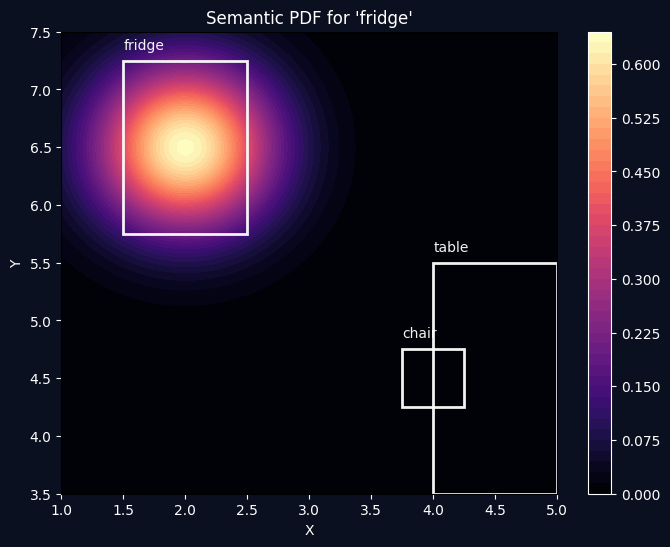
\includegraphics[width=0.95\linewidth]{figures/fridge_semantic.png}
        \caption{Semantic Grounding}
        \label{fig:fridge_semantic}
    \end{subfigure}\hfill
    \begin{subfigure}[t]{0.45\linewidth}
        \centering
        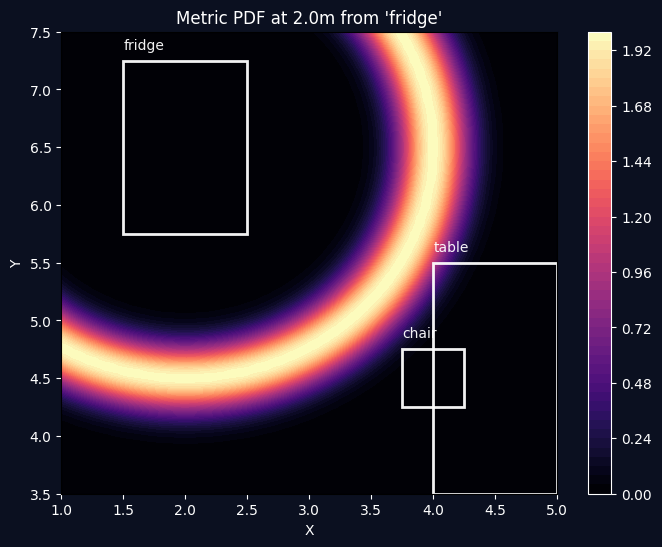
\includegraphics[width=0.95\linewidth]{figures/fridge_metric.png}
        \caption{Metric Kernel}
        \label{fig:fridge_metric}
    \end{subfigure}

    \vspace{0.3em}

    \begin{subfigure}[t]{0.45\linewidth}
        \centering
        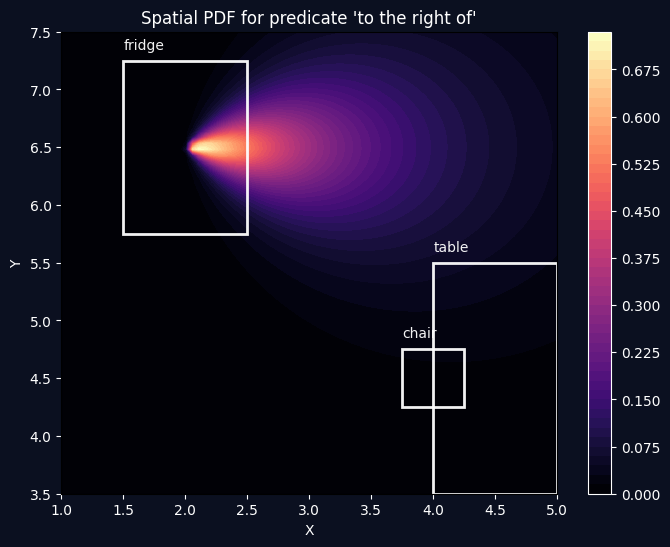
\includegraphics[width=0.95\linewidth]{figures/fridge_spatial.png}
        \caption{Spatial Kernel}
        \label{fig:fridge_spatial}
    \end{subfigure}\hfill
    \begin{subfigure}[t]{0.45\linewidth}
        \centering
        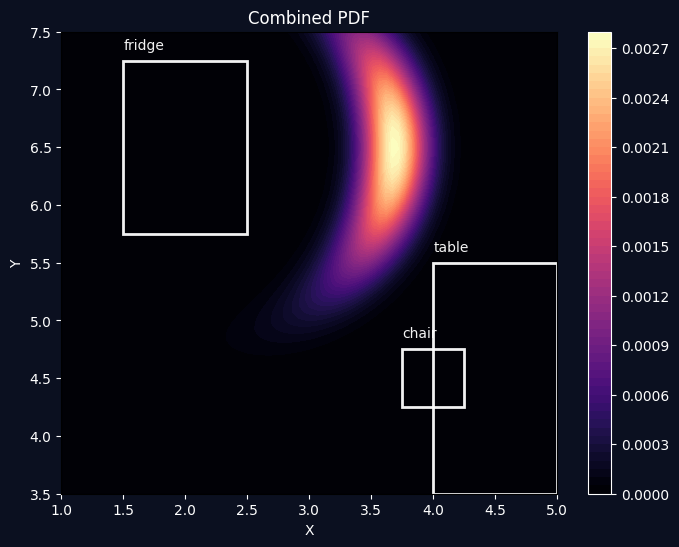
\includegraphics[width=0.95\linewidth]{figures/fridge_composed.png}
        \caption{Composed Distribution}
        \label{fig:fridge_composed}
    \end{subfigure}

    \caption{MAPG grounding for the query ``Where is \SI{2}{m} to the right of the fridge?'' Semantic grounding (a) identifies the fridge instance; the metric kernel (b) enforces the \SI{2}{m} radial offset; the directional kernel (c) captures ``right of'' as a vMF distribution in the fridge's local frame. Their log-space composition (d) yields a planner-ready goal distribution peaking $0.07\,\mathrm{m}$ from the ground truth.}
    \label{fig:fridge_kernels_row}
\end{figure}

%\opnote{My main complaint here is that the term agent has a specific meaning...}

\noindent$\!\!$\textbf{1) \uline{The Orchestrator}} parses a free-form instruction into Spatial Description Clauses (SDCs)~\cite{kollar2010toward}: a target entity, anchor objects with optional modifiers and explicit metric distances, and a \emph{composition logic} label. Crucially, the Orchestrator classifies each spatial predicate as either camera-relative (\texttt{near}, \texttt{between}) or intrinsic object-centric (\texttt{intrinsic\_front}, \texttt{intrinsic\_back}, \texttt{intrinsic\_left}, \texttt{intrinsic\_right}), enabling downstream kernel computation to select the correct reference frame. For ``Where is $2\,\mathrm{m}$ to the right of the fridge?'' it produces: anchor=\texttt{fridge}, composition\_logic=\texttt{intrinsic\_right}, metric=\texttt{2.0\,m}. Multi-clause instructions yield a conjunction of SDCs, each resolved independently and composed downstream.
%\opnote{The methods section is too mechanistic...}

\noindent$\!\!$\textbf{2) \uline{The Grounding Agent}} resolves each anchor label to a concrete object instance in $\Gamma$. Given a referent like ``fridge,'' it combines: (i) semantic equivalence matching (``couch'' = ``sofa'') against scene-graph labels, (ii) visual verification via a VLM query over base64-encoded egocentric images, and (iii) a spatial salience prior (proximity, visibility). Candidates rejected by the Verifier are blacklisted in the shared failure history and excluded from subsequent queries. A belief distribution $B_t(o)$ over candidate instances is maintained on the blackboard; the agent iterates across multiple views until sufficient confidence is reached, making it a genuine evidence-accumulating agent.

\rev{\noindent$\!\!$\textbf{3) \uline{Spatial Kernel Estimator}} (Spatial Agent)}: Once anchor $o_r$ with pose $t_o \in \mathbb{R}^3$ is resolved, MAPG instantiates three analytic kernels whose log-likelihoods sum in closed form (Fig.~\ref{fig:fridge_kernels_row}):

\noindent\textbf{Semantic kernel}: a $3$D Gaussian centered at the anchor: $\ell_{\text{sem}}(x) = -\tfrac{1}{2\sigma_s^2}\|x - t_o\|^2$.

\noindent\textbf{Metric kernel}: a radial Gaussian over distance from the anchor: $\ell_{\text{met}}(x) = -\tfrac{1}{2\sigma_m^2}(\|x-t_o\| - d_0)^2$, \rev{where $d_0$ is parsed from the query by the Orchestrator and $\sigma_m$ is a system tolerance.}

\noindent\textbf{Spatial (directional) kernel}: a von Mises-Fisher distribution~\cite{tellex2011symbolgrounding} in the anchor's local frame:
$\ell_{\text{dir}}(x;\theta_0,\phi_0,\kappa)=\kappa\bigl(R_o\,m(\theta_0,\phi_0)\bigr)^\top\widehat{(x-t_o)}$,
\rev{where $R_o$ maps from the anchor's local to world frame, $\widehat{(x-t_o)}$ is the unit direction from anchor to $x$, and $\kappa$ is a system concentration parameter.}

\rev{\noindent\textbf{Composition and the role of the semantic kernel.}
The three log-likelihoods sum and are normalized over $\Omega_{\text{free}}$. The semantic and metric kernels, however, are not independent: $\ell_{\text{sem}}$ is centred \emph{on} the anchor while $\ell_{\text{met}}$ peaks at radius $d_0$ \emph{from} it, so summing all three shrinks the composed mode inward. Along the modal ray $\ell_{\text{dir}}$ is constant in $r$, giving a closed form for the peak radius
\begin{equation}
r^{\star} = d_0\,\frac{\sigma_s^{2}}{\sigma_s^{2}+\sigma_m^{2}} \;<\; d_0 ,
\label{eq:shrinkage}
\end{equation}
a systematic underestimate of the commanded offset. With $\sigma_s$ scaled to the anchor extent ($\sigma_s=0.5\,\text{max-dim}$) and $\sigma_m=0.30\,\mathrm{m}$, a $2\,\mathrm{m}$ offset from a typical $0.8\,\mathrm{m}$ fridge would peak at $1.28\,\mathrm{m}$, an error of $0.72\,\mathrm{m}$ induced purely by the composition.
We therefore treat the semantic kernel as an \emph{anchor-selection} term rather than a goal-placement term. In O-O mode it scores candidate instances and all three kernels apply. In O-W mode, where the goal is a free-space waypoint and the anchor is already resolved, the semantic term carries no information about \emph{where along} the offset the goal lies, so we flatten it ($\sigma_s\!\to\!\infty$) and compose
\begin{equation}
\log P(x) = \ell_{\text{met}} + \ell_{\text{dir}},
\label{eq:ow-composition}
\end{equation}
which by Eq.~\ref{eq:shrinkage} recovers $r^{\star}=d_0$ exactly. This is what makes the metric constraint hold to centimetre accuracy; naively multiplying all three experts would not.}

\rev{\noindent\textbf{VLM parameter inference.} The Spatial Kernel Estimator prompts a VLM with the anchor label, current agent pose and yaw $\psi$, scene graph context, and an egocentric image. The VLM predicts the camera-relative azimuth $\theta_{\text{cam}}$ toward the goal region; the system converts this to a world-frame direction $\theta_0 = (\psi + \theta_{\text{cam}}) \bmod 2\pi$. For predicates classified as \texttt{intrinsic\_*} by the Orchestrator, $\theta_0$ is further resolved using the anchor's stored orientation rather than camera frame, enabling the commonsense subset's frame-of-reference predicates. This design asks the VLM only to answer ``in which camera direction is the goal?'' (a task VLMs handle well) while the coordinate transform and metric enforcement are handled analytically.}

\rev{\noindent$\!\!$\textbf{4) \uline{Cascading Spatial Kernels.}}
For compound instructions, one kernel triplet is instantiated per clause, each anchored to its resolved referent. All log-likelihoods are summed and renormalized, implementing a Product of Experts~\cite{hinton2002poe} whose peak satisfies the conjunction of all spatial constraints.}

\rev{\noindent$\!\!$\textbf{5) \uline{Verifier and Planner.}}
The \emph{Verifier} performs four checks on each proposed grounding: (i) orchestrator logic soundness, (ii) egocentric alignment ($\theta_{\text{cam}}$ consistent with what is visible in the image), (iii) semantic label flexibility (``sofa'' accepted for ``couch''), and (iv) absence of visual hallucination. A FAIL result appends structured feedback to the global failure history and re-triggers the Grounding Agent or Spatial Kernel Estimator as appropriate, forming a closed refinement loop. Waypoints that pass verification are forwarded to the \emph{Planner} (RRT*~\cite{karaman2011sampling}) for trajectory generation.}
